\documentclass[]{../template/Report}%方括号内写yuxi即生成预习报告
\settemplatedir{../template/}%设置模板路径

\exname{} %实验名称
\extable{} %实验桌号
\instructor{} %指导教师
\class{} %班级
\name{} %姓名
\stuid{} %学号

\nyear{} %年
\nmonth{} %月
\nday{} %日
\nweekday{} %星期几
\daypart{}%上午/下午

\redate{} %如有实验补做,补做日期
\resitu{} %情况说明:

\begin{document}
\maketitle

\section{预习报告}
\subsection{实验综述}

\subsubsection{自组电桥测未知电阻}
惠斯登电桥电路如\cref{huisideng}所示。$R_1,R_2$为定值电阻,$R_x$为待测电阻,$R_s$为可变电阻。测量时,调节$R_x$使检流计$G$示数为$0$。此时$U_B=U_D$,根据电路分析原理$I_1R_1=I_2R_2$且$I_1R_x=I_2R_s$,解得
\[
    R_x = \frac{R_1}{R_2} R_s
\]
其中系数$\frac{R_1}{R_2}$称为倍率。实验中比率的设定应保证结果有4位有效数字。

如果交换$R_x,R_s$的位置再次测量,结果为$R_x'=\frac{R_2}{R_1}R_s'$。取两次结果的平均$\overline{R_x} = \sqrt{R_sR_s'}$作为结果,就消除了$R_1,R_2$的误差对结果的影响。该方法称为交换法。本次使用交换法。
\begin{figure}[H]
    \centering
    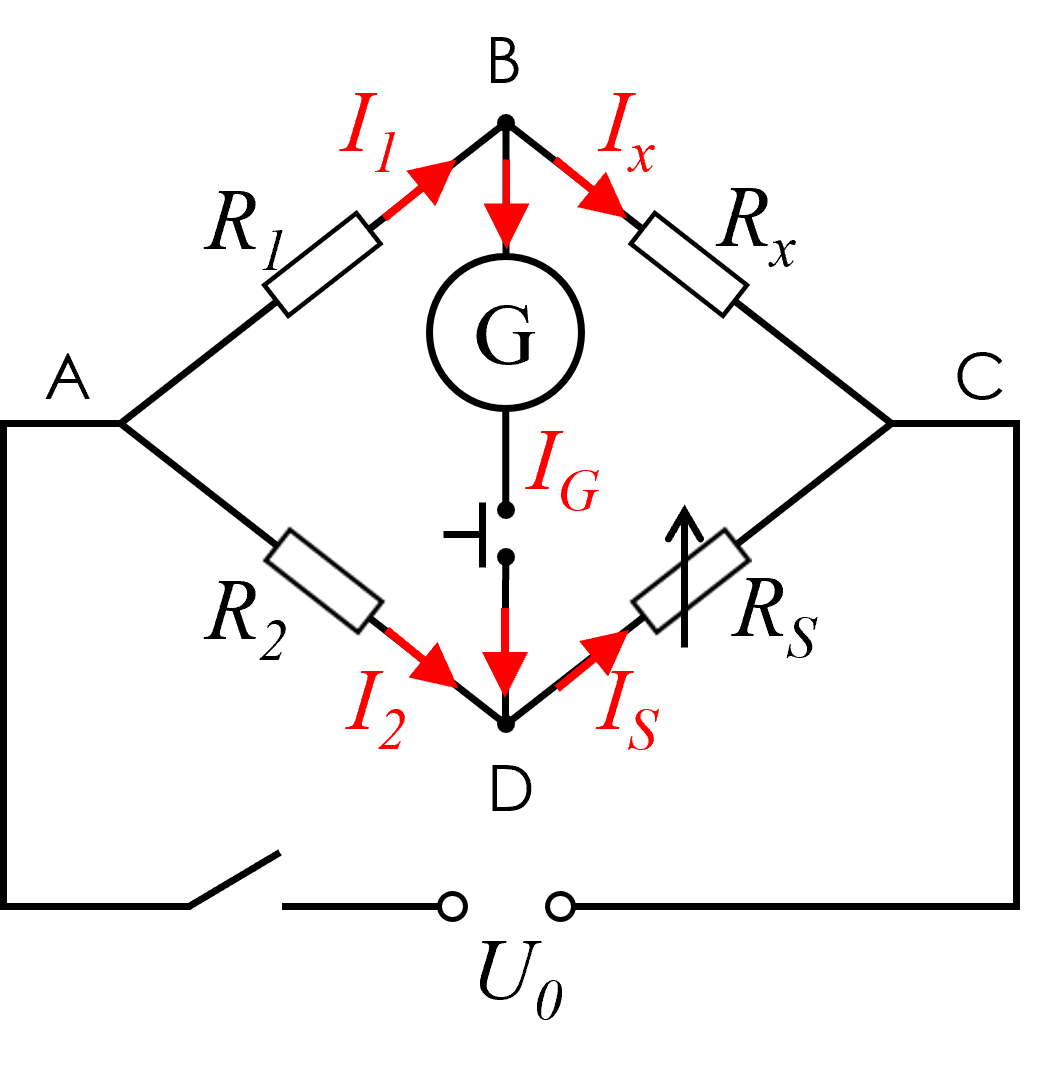
\includegraphics[width=0.4\textwidth]{huisideng.png}
    \caption{惠斯登电桥电路图}
    \label{huisideng}
\end{figure}


该实验的相对误差由两方面构成,由$R_s$产生的相对误差和两次测定中检流计读数产生的相对误差。前者的计算式是:
\[\frac{\Delta R_x}{R_x} = \frac{1}{2} \sqrt{\left(\frac{\Delta R_s}{R_s}\right)^2 + \left(\frac{\Delta R'_s}{R'_s}\right)^2} \approx \frac{\Delta R_s}{R_s}\]

其中$\frac{\Delta R_s}{R_s}$由仪器误差决定。当$R_s$使用十进位转盘直流电阻箱时,$\frac{\Delta R_s}{R_s} = \pm \left(a+b\frac{m}{R_x}\right)\%$,其中$a$是电阻箱精确度等级,$b$是与精确度等级有关的系数,$m$是使用电阻箱的总盘数。一般常用的 0.1 级十进位转盘电阻箱 $a=0.1$,$b=0.2$,则
\[\Delta R_s = \pm (0.001 R_s + 0.002 m)\]

为计算后一个相对误差,定义电桥灵敏度
\[S = \frac{\Delta d}{\Delta R_s /R_s}\]
其中$\Delta R_s$为电阻箱的改变量,$\Delta d$为改变$R_s$引起检流计$G$的偏转格数。$S$可通过实验测得。

测得电桥灵敏度后,在电桥灵敏度定义式中令$\Delta d = 0.2$(人眼察觉到的极限为0.2小格),得到由检流计初次测量产生的相对误差
\[\frac{\Delta R_{s\text{检}}}{R_{s\text{检}}} = \frac{0.2}{S}\]

综合起来,得待测电阻的相对不确定度
\[E = \frac{\Delta R_x}{\overline{R_x}} = \sqrt{ \left(\frac{\Delta R_1}{R_1}\right)^2 + \left(\frac{\Delta R_{s\text{检}}}{R_{s\text{检}}}\right)^2} = \sqrt{\left(0.001+ \frac{0.002m}{R_s}\right)^2 + \left(\frac{0.2}{S}\right)^2}\]

不确定度
\[u = \Delta R_x = E \overline{R_x}\]

最终结果表示为
\[R_x = \overline{R_x} \pm \Delta R_x\]

本实验需要处理的数据包括:电桥的倍率$\frac{R_1}{R_2}$,交换法测量的结果$R_s,R'_s$,电桥灵敏度$S = \frac{\Delta d}{\Delta R_s /R_s}$及计算公式的各参数,待测电阻相对误差$E$、不确定度$u$和测量结果$R_x$。
\subsubsection{用QJ\_23型盒式惠斯登电桥测电阻离散度}

打开盒式电桥,选择工作电源,将指针调零。依次测量待测电阻盘上8个等值电阻,选取适当的倍臂,确保测量结果有效数字达4位,计算这批电阻的离散度$\frac{S}{\overline{R_x}} \times 100\%$。

其中,$\overline{R_x}$是所有电阻的均值,标准偏差由贝塞尔公式给出$S = \sqrt{\frac{1}{n-1} \left[\sum_{k=1}^{n}(x_k - \overline{x})^2\right]}$。

本实验需要处理的数据包括各待测电阻值,电阻均值,标准偏差,离散度。


\subsection{实验重点}
\begin{enumerate}
    \item 掌握惠斯登电桥工作原理及其特点,学会自组电桥测量未知电阻;
    \item 理解不确定性和误差分析的方法和技巧;
    \item 掌握正确使用盒式惠斯登电桥测量电阻的方法;
    \item 掌握数据标准偏差和离散度的计算方法。
\end{enumerate}
\subsection{实验难点}
\begin{enumerate}
    \item 熟练组装和使用惠斯登电桥;
    \item 分析惠斯登电桥的特性;
    \item 掌握不确定度和误差分析的方法;
    \item 掌握标准偏差、离散度的计算方法。
\end{enumerate}

\begin{fullreportonly}
% \section{原始数据}
% \begin{figure}[H]
%     \centering
%     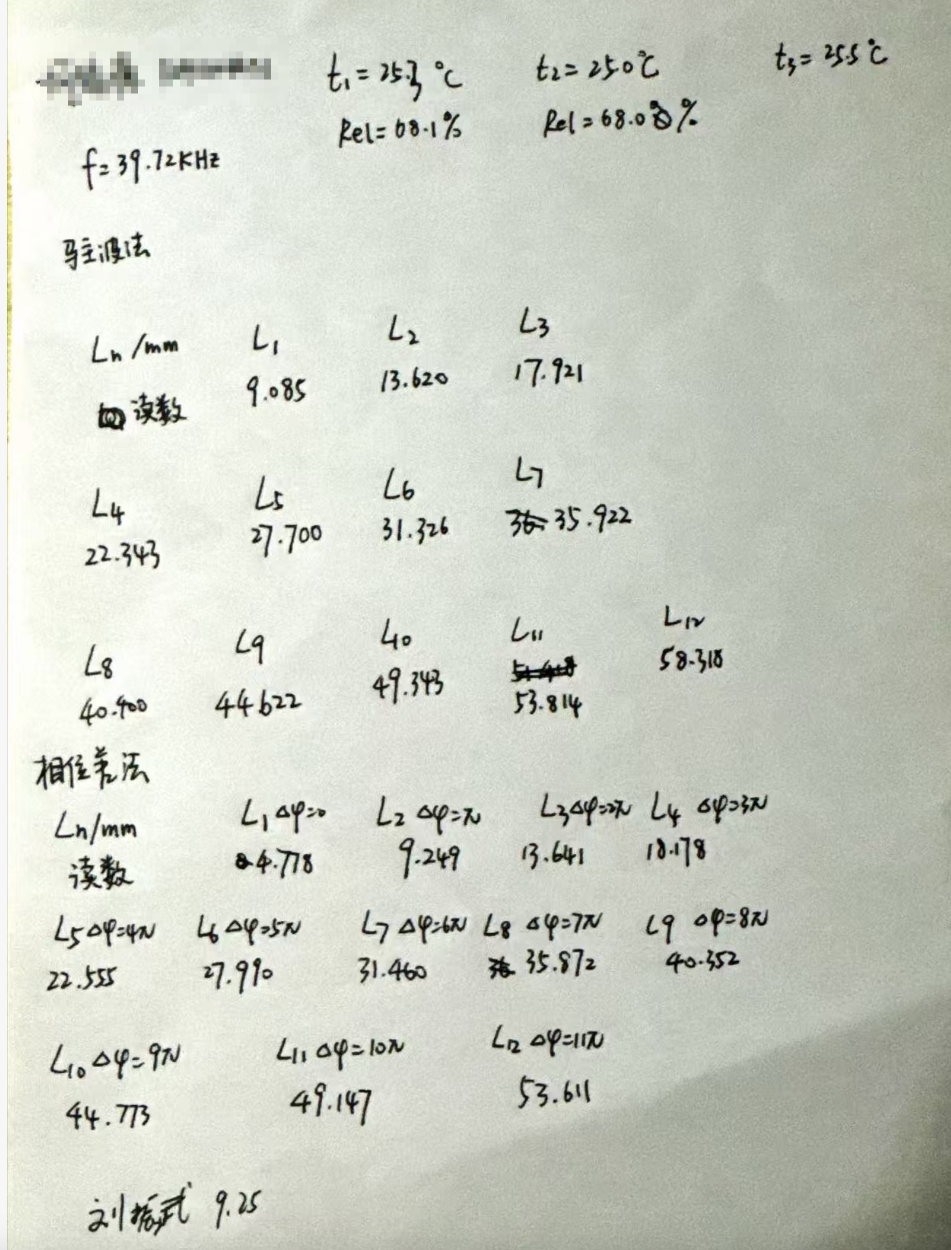
\includegraphics[width=0.8\textwidth]{data.jpg}
%     \caption{原始数据记录}
%     \label{data}
% \end{figure}
\section{结果与分析}
\subsection{数据处理与结果}
\subsubsection{交换法测量未知电阻}
首先,组装电桥,用交换法测量未知电阻。为得到尽可能多的有效数字,取$R_1=R_2 = 1000 \si{\ohm}$。
测得$R_s = \SI{219.9}{\ohm},R_s = \SI{219.8}{\ohm}$。
可知此时倍率为$\frac{R_1}{R_2} = 1 $,待测电阻阻值为
\[\overline{R_x} = \sqrt{R_s R'_s} = \SI{219.8}{\ohm}\]

再测量电桥灵敏度,在$R_s$为$\SI{219.9}{\ohm}$时,调整$\Delta R_s = \SI{0.1}{\ohm}$,此时指针偏转了$\Delta d = 13$小格,则电桥灵敏度为
\[S = \frac{\Delta d}{\frac{\Delta R_s}{R_s}} = \frac{13}{\frac{0.1}{219.9}} = 28587\]

$R_x$ 相对不确定度
\[E = \frac{\Delta R_x}{\overline{R_x}} = \sqrt{\left(0.001+ \frac{0.002m}{R_s}\right)^2 + \left(\frac{0.2}{S}\right)^2} = 0.10\% \]

则 $\Delta R_x = E \cdot \overline{R_x} = \SI{0.2}{\ohm}$。$R_x = (\overline{R_x} \pm \Delta R_x)\,\si{\ohm} = (219.8 \pm 0.2)\,\si{\ohm}$。
\subsubsection{用QJ\_23型盒式惠斯登电桥测电阻离散度}
实验中选择倍率为$0.1$,利用直接法就能算出各待测电阻阻值如\cref{yiduidianzu}所示。
\begin{table}[H]
    \caption{测得各电阻数据}
    \centering
    \begin{tabular}{C{0.1\textwidth}C{0.08\textwidth}C{0.08\textwidth}C{0.08\textwidth}C{0.08\textwidth}C{0.08\textwidth}C{0.08\textwidth}C{0.08\textwidth}C{0.08\textwidth}}
        \toprule
        待测电阻 & $R_1$ & $R_2$ & $R_3$ & $R_4$ & $R_5$ & $R_6$ & $R_7$ & $R_8$ \\
        \midrule
        电阻/$\si{\ohm}$ & 687.8 & 687.0 & 680.1 & 675.6 & 680.1 & 683.1 & 675.2 & 679.4 \\
        \bottomrule
    \end{tabular}
    \label{yiduidianzu}
\end{table}
这组电阻的均值为$\overline{R_x} = \frac{1}{8}\sum_{i=1}^{8} R_{i} = \SI{681.0}{\ohm}$,标准偏差为$S = \sqrt{\frac{1}{8-1}\sum_{i=1}^{8}(R_{i} - \overline{R_x})^2} = \SI{4.7}{\ohm}$,则离散度为
\[\frac{S}{\overline{R_x}} \times 100\% = 0.69\% \]


\subsection{误差分析}
\begin{enumerate}
    \item 人眼观察检流计时,存在视觉误差,导致测量不准;
    \item 检流计很难准确调零,影响对零偏的观察;
    \item 电阻箱标称值和实际值存在偏差,导致测出的$\overline{R_x}$产生误差;
    \item 电阻箱分度值较低,无论怎么调整都不能使检流计严格达到零偏,限制了测量结果的准确性;
    \item 观察到环境因素乃至导线位置都会影响检流计偏转情况,说明检流计偏转情况并不严格准确,从而影响结果。
\end{enumerate}
\subsection{实验探讨}
本次实验使用经典的惠斯登电桥法测量电阻,并使用交换法有效降低误差。
不仅使我对电路原理和实验技巧有了更深刻的认识,
还使我的数据处理、误差分析和有效数字分析的能力得到显著提升。
\section{思考题}
\subsection{为什么用惠斯登电桥测电阻比伏安法测量的准确度高?用电桥法测电阻产生误差的主要因素是什么?}

\subsubsection{准确高的原因}
\begin{enumerate}
    \item \textbf{避免电表内阻的影响:} 伏安法需同时测量电流和电压,电表的内阻会引入系统误差(如电流表分压、电压表分流),无论采用内接法还是外接法,都无法完全消除电表内阻的影响;而电桥法在平衡时无需直接测量电流或电压,避免了电表内阻的影响。
    
    \item \textbf{最大限度避免读数误差:} 电桥法中,只要$R_s$有微小变化,检流计将变化很大,理论上误差大部分来源于电阻箱有限的精度;但伏安法中,电表读数就会产生很大误差;

    \item \textbf{电源稳定性:} 伏安法对电源稳定性要求不高。电源电压的波动会影响桥路失衡时的电流,但一旦调节到平衡点(检流计指零),电源电压的变化不会改变平衡条件。
\end{enumerate}
\subsubsection{用电桥法测电阻产生误差的主要因素}
\begin{enumerate}
    \item \textbf{桥臂电阻的误差:} 测量结果$ R_x = \frac{R_1}{R_2} \cdot Rs $的精度直接依赖于三个已知电阻$R_1, R_2, R_s$的精度。如果这些电阻的标称值不准、随时间漂移或因温度变化而改变,会直接导致系统误差。
    \item \textbf{电阻箱精度有限:} 实验中,无论如何调节电阻箱,检流计都无法严格零偏,说明电阻箱精度限制了结果的精度;
    \item \textbf{环境因素的影响:} 热量、电磁效应等环境因素会干扰检流计和电阻阻值等,从而造成误差。
\end{enumerate}
\subsection{为了提高电桥测量灵敏度,应采取哪些措施?为什么?}
\begin{enumerate}
    \item 在允许范围内增大电源电压,这样在电桥不平衡时通过检流计电流更大,从而更易判断电桥是否平衡;
    \item 根据情况选择合适的比率臂,从而得到尽可能多的有效数字,电阻箱给出的$R_s$有效数字越多,结果有效数字就越多,因此应调整比率使电阻箱使用最高位的电阻;
    \item 选择灵敏度更高的检流计,因为检流计越灵敏,越能判断出电桥是否平衡;
    \item 选用分度值更小的电阻箱,与第2点类似,这样会得出更多有效数字,也更容易让电桥严格平衡。
\end{enumerate}
\subsection{用电桥测电阻时,若线路接通后检流计指针总是往一个方向偏转或总不偏转,试分析是什么原因?}
总是往一个方向偏转,可能是电桥的比率臂(倍率)选择不合理,导致偏差过大(比率臂与标准电阻$R_s$的乘积远大于或小于被测电阻$R_x$);可能是电阻箱阻值范围选择不当,使电桥无法平衡;也可能是电路连接有误,出现了短路或断路。

总不偏转。可能是电路连接有误,如电桥回路中某处(如导线、开关、电阻)完全断开或检流计本身被短路;也可能是电源未接通或电压过小,或仪器本身出现故障。
\subsection{惠斯登电桥比率臂选取的原则是什么?为什么要这样选取?}
\begin{enumerate}
    \item 使得$R_s$的调节范围满足$\frac{R_1}{R_2}R_s$能取到$R_x$的估测值,否则电桥无法平衡;
    \item 在保证安全的前提下,应尽可能多地使用电阻箱的有效位数,因为这样能提高测量结果的有效数字位数;
    \item 最好使比率臂为$10$的整数次幂,以避免复杂计算导致的舍入。
\end{enumerate}


\subsection{如何使用自组电桥测量电表内阻(注意电表所能允许通过的最大电流)?根据电桥平衡的特点,可否将桥路中的检流计去掉,换成行测电表判别电桥的平衡?}

电路和原理和本次实验“用自组电桥测量未知电阻”相同,只需把$R_x$换为待测电表即可,因为电表实际就相当于一块电阻。但需要注意通过的电流不能超过电表所能允许通过的最大电流。这可以通过根据电流表的最大电流和内阻估算值选择$\varepsilon$和$R_1$达到,或也可以为电表串联一保护电阻。

理论可以去掉检流计而只根据行测电表判断电桥平衡。在\cref{huisideng}中,如果电桥上的开关无论是否闭合,行测电表示数都一致,就可认为电桥中没有电流通过。因为该现象说明B、D两点等势,从而电桥平衡。
不过由于行测电表灵敏度较低,$R_s$在一定范围内变化时电表偏转都不会发生明显变化,因此这样误差将较大。

\end{fullreportonly}
\insertnotes
\end{document}